% -*- program: xelatex -*-

\documentclass[12pt
, t
% , draft
]{beamer}
%%% ------------------------------------------------------------------------
% packages
\usepackage{tikz}
\usetikzlibrary{shapes.geometric, arrows, positioning, shapes, backgrounds}
\usepackage{graphicx}
\usepackage{lmodern}
\usepackage{adjustbox}
% conditional (for figures)
\usepackage{etoolbox}
\usepackage{amsfonts}

\usepackage{fontspec}
\usepackage{fontawesome}

\usepackage{tikz}
\usepackage{adjustbox}

\usepackage{subcaption} % side-by-side figures
\usepackage{hyperref}

\newtoggle{dark}

%%% ------------------------------------------------------------------------
% Theming (dark or white)
\usetheme{default}
\useoutertheme[subsection=false]{miniframes}

% move navigation to footer
\setbeamertemplate{headline}{}
\makeatletter
\setbeamertemplate{footline}
  {%
  \begin{beamercolorbox}{section in head/foot}
    \vskip2pt\insertnavigation{\paperwidth}\vskip5pt
  \end{beamercolorbox}%
  }
\makeatother


% no navigation bar
\beamertemplatenavigationsymbolsempty

% switch!
\toggletrue{dark}
% \togglefalse{dark}

\iftoggle{dark}{%
	% some colors
	\definecolor{foreground}{RGB}{255,255,255}
	\definecolor{background}{RGB}{24,24,24}
	\definecolor{title}{RGB}{127,185,220}
	\definecolor{gray}{RGB}{160,160,160}
	\definecolor{hilight}{RGB}{250, 108, 0}
	\setbeamercolor{section in head/foot}{fg = title}
	% set colors for titles, etc.
	\setbeamercolor{titlelike}{fg=title}
	\setbeamercolor{subtitle}{fg=title}
	\setbeamercolor{institute}{fg=gray}
	\setbeamercolor{normal text}{fg=foreground,bg=background}
	% % set colors for itemize
	\setbeamercolor{item}{fg=title} % color of bullets
	\setbeamercolor{subitem}{fg=gray}
	\setbeamercolor{itemize/enumerate subbody}{fg=gray}
}{
	% some colors
	\definecolor{foreground}{RGB}{0, 0, 0}
	\definecolor{background}{RGB}{255,255,255}
	\definecolor{title}{RGB}{107,174,214}
	\definecolor{gray}{RGB}{116,116,116}
	\definecolor{hilight}{RGB}{228, 97, 0}
	\setbeamercolor{section in head/foot}{fg = title}
	% set colors
	\setbeamercolor{titlelike}{fg=title}
	\setbeamercolor{subtitle}{fg=title}
	\setbeamercolor{institute}{fg=gray}
	\setbeamercolor{normal text}{fg=foreground,bg=background}
	% set colors for itemize
	\setbeamercolor{item}{fg=foreground} % color of bullets
	\setbeamercolor{subitem}{fg=gray}
	\setbeamercolor{itemize/enumerate subbody}{fg=gray}
}


%%% ------------------------------------------------------------------------
% Meta
\title{Statistical Ecotoxicology \\ - Improving the utilization of data for ecological risk assessment}   
\author{Eduard Szöcs} 
\institute{Institute for Environmental Sciences, University of Koblenz-Landau}
\date{Landau, 22.09.2016}



%%% ------------------------------------------------------------------------
\begin{document}
\begin{frame}
\titlepage
\end{frame}


%%% ---------------------------------------------------------------------------
\section{Statistical Ecotoxicology} 
\subsection{}
\begin{frame}
\frametitle{My field of research is somewhere between...}
	\center
	
\includegraphics[width = 0.8\textwidth]{fig/wc_all.png} \\
	\mbox{... Eco(-toxico)logy, Data Analysis \& Programming}
\end{frame}


\subsection{}
\begin{frame}[plain]
	\begin{tikzpicture}[overlay, remember picture]
	\node[anchor=center] at (current page.center) {
		\begin{beamercolorbox}[center]{title}
	     \Huge Statistical Ecotoxicology
	  \end{beamercolorbox}};
	\end{tikzpicture}
\end{frame}


\begin{frame}
\frametitle{Current use in ecotoxicology}
	\begin{itemize}
		\item<1->{Ecological risk assessment (ERA) relies on statistics}
		\item<2->{Experiments with low replication}
		\item<3->{Usually analysed using Linear Models of transformed data}
		\item<3->{Null Hypothesis Significance Testing (=> NOEC)}
	\end{itemize}

	\only<1>{
	\begin{adjustbox}{max totalsize={.9\textwidth}{.6\textheight},center}
	\begin{tikzpicture}[node distance = 2cm, auto]
		\usetikzlibrary{shapes, arrows, positioning, calc}
		% Define elements
		\tikzstyle{line} = [draw, -latex', ultra thick]
		\tikzstyle{block} = [rectangle, draw, 
		    text width=5em, text centered, rounded corners, minimum height=4em]
		\tikzstyle{paper} = [circle, draw, fill=gray!85, fill opacity=0.4, text opacity=1,  font = \bf, minimum width=2.5cm]
		\tikzstyle{textbf} = [text centered, font = \bf\Large]
		%% Effects
		\node [name = exp, block, minimum width=2cm] {Experiment} ;
		\node [name = stat, block, minimum width=2cm, right=1cm of exp, fill=hilight] {Data / Statistics} ;
	    \node [name = eff, block, 
			minimum width=6.4cm, 
			minimum height=3.5cm, 
		below left=5mm of exp.west, anchor = west] {} ;
		\node[textbf, below right=10mm and 5mm of exp, anchor = south]{Effects};

		%% Exposure
	  	\node [name = prop, block, minimum width=2cm, below=4cm of exp] {Data / Properties} ;
		\node [name = model, block, minimum width=2cm, right=1cm of prop] {Models} ;
		\node [name = expo, block, 
			minimum width=6.4cm, 
			minimum height=3.5cm, 
			below = 15mm of eff] {} ;
		\node[textbf, above=-2mm of expo, anchor = north]{Exposure};

		%% Risk Assessment
		\node [name = risk, block, below right=0.75cm and 1cm of stat,
	       minimum width=5cm, 
			minimum height=2.5cm, 
			font = \bf\large,
			align = center,
	       text width = 3cm] {Ecological Risk\\  Assessment};
	% arrows
		\path [line] (exp) -- (stat);
		\path [line] (prop) -- (model);
		\path [line] (eff) -| (risk);
		\path [line] (expo) -| (risk);
	\end{tikzpicture}
	\end{adjustbox}
	}

	\only<3>{
		\begin{center}
		\colorbox{white}{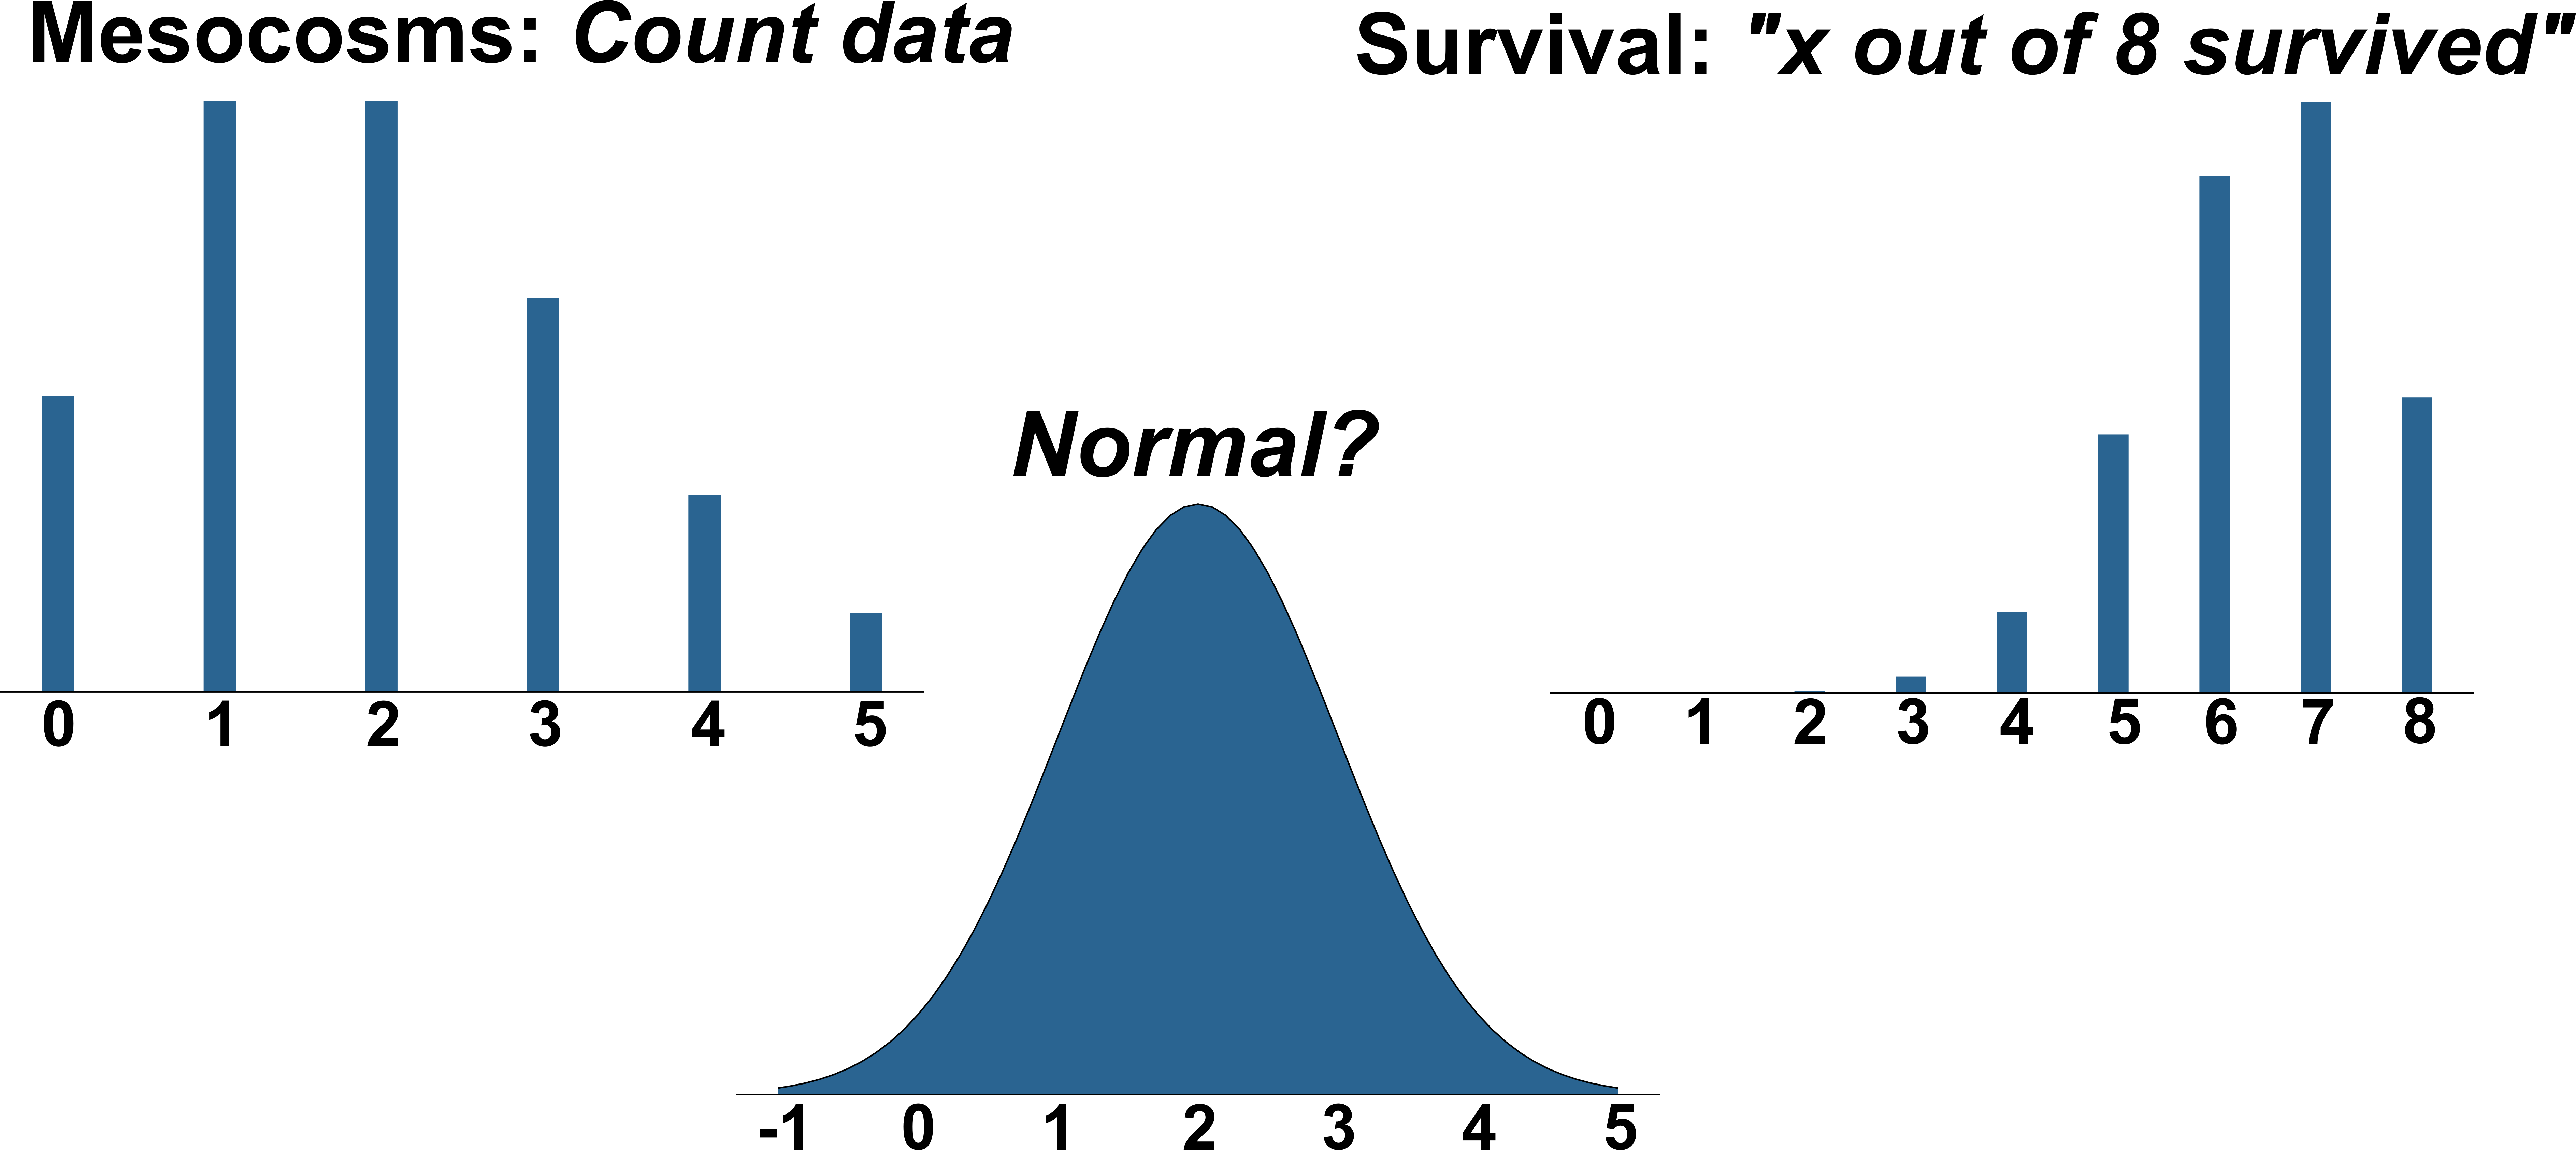
\includegraphics[width=0.8\textwidth]{fig/distr.png}}
		\end{center}
	}
\end{frame}


\begin{frame}
	\frametitle{Statistical Power in current experimental designs in ecotoxicology is unacceptably low}
	\center
	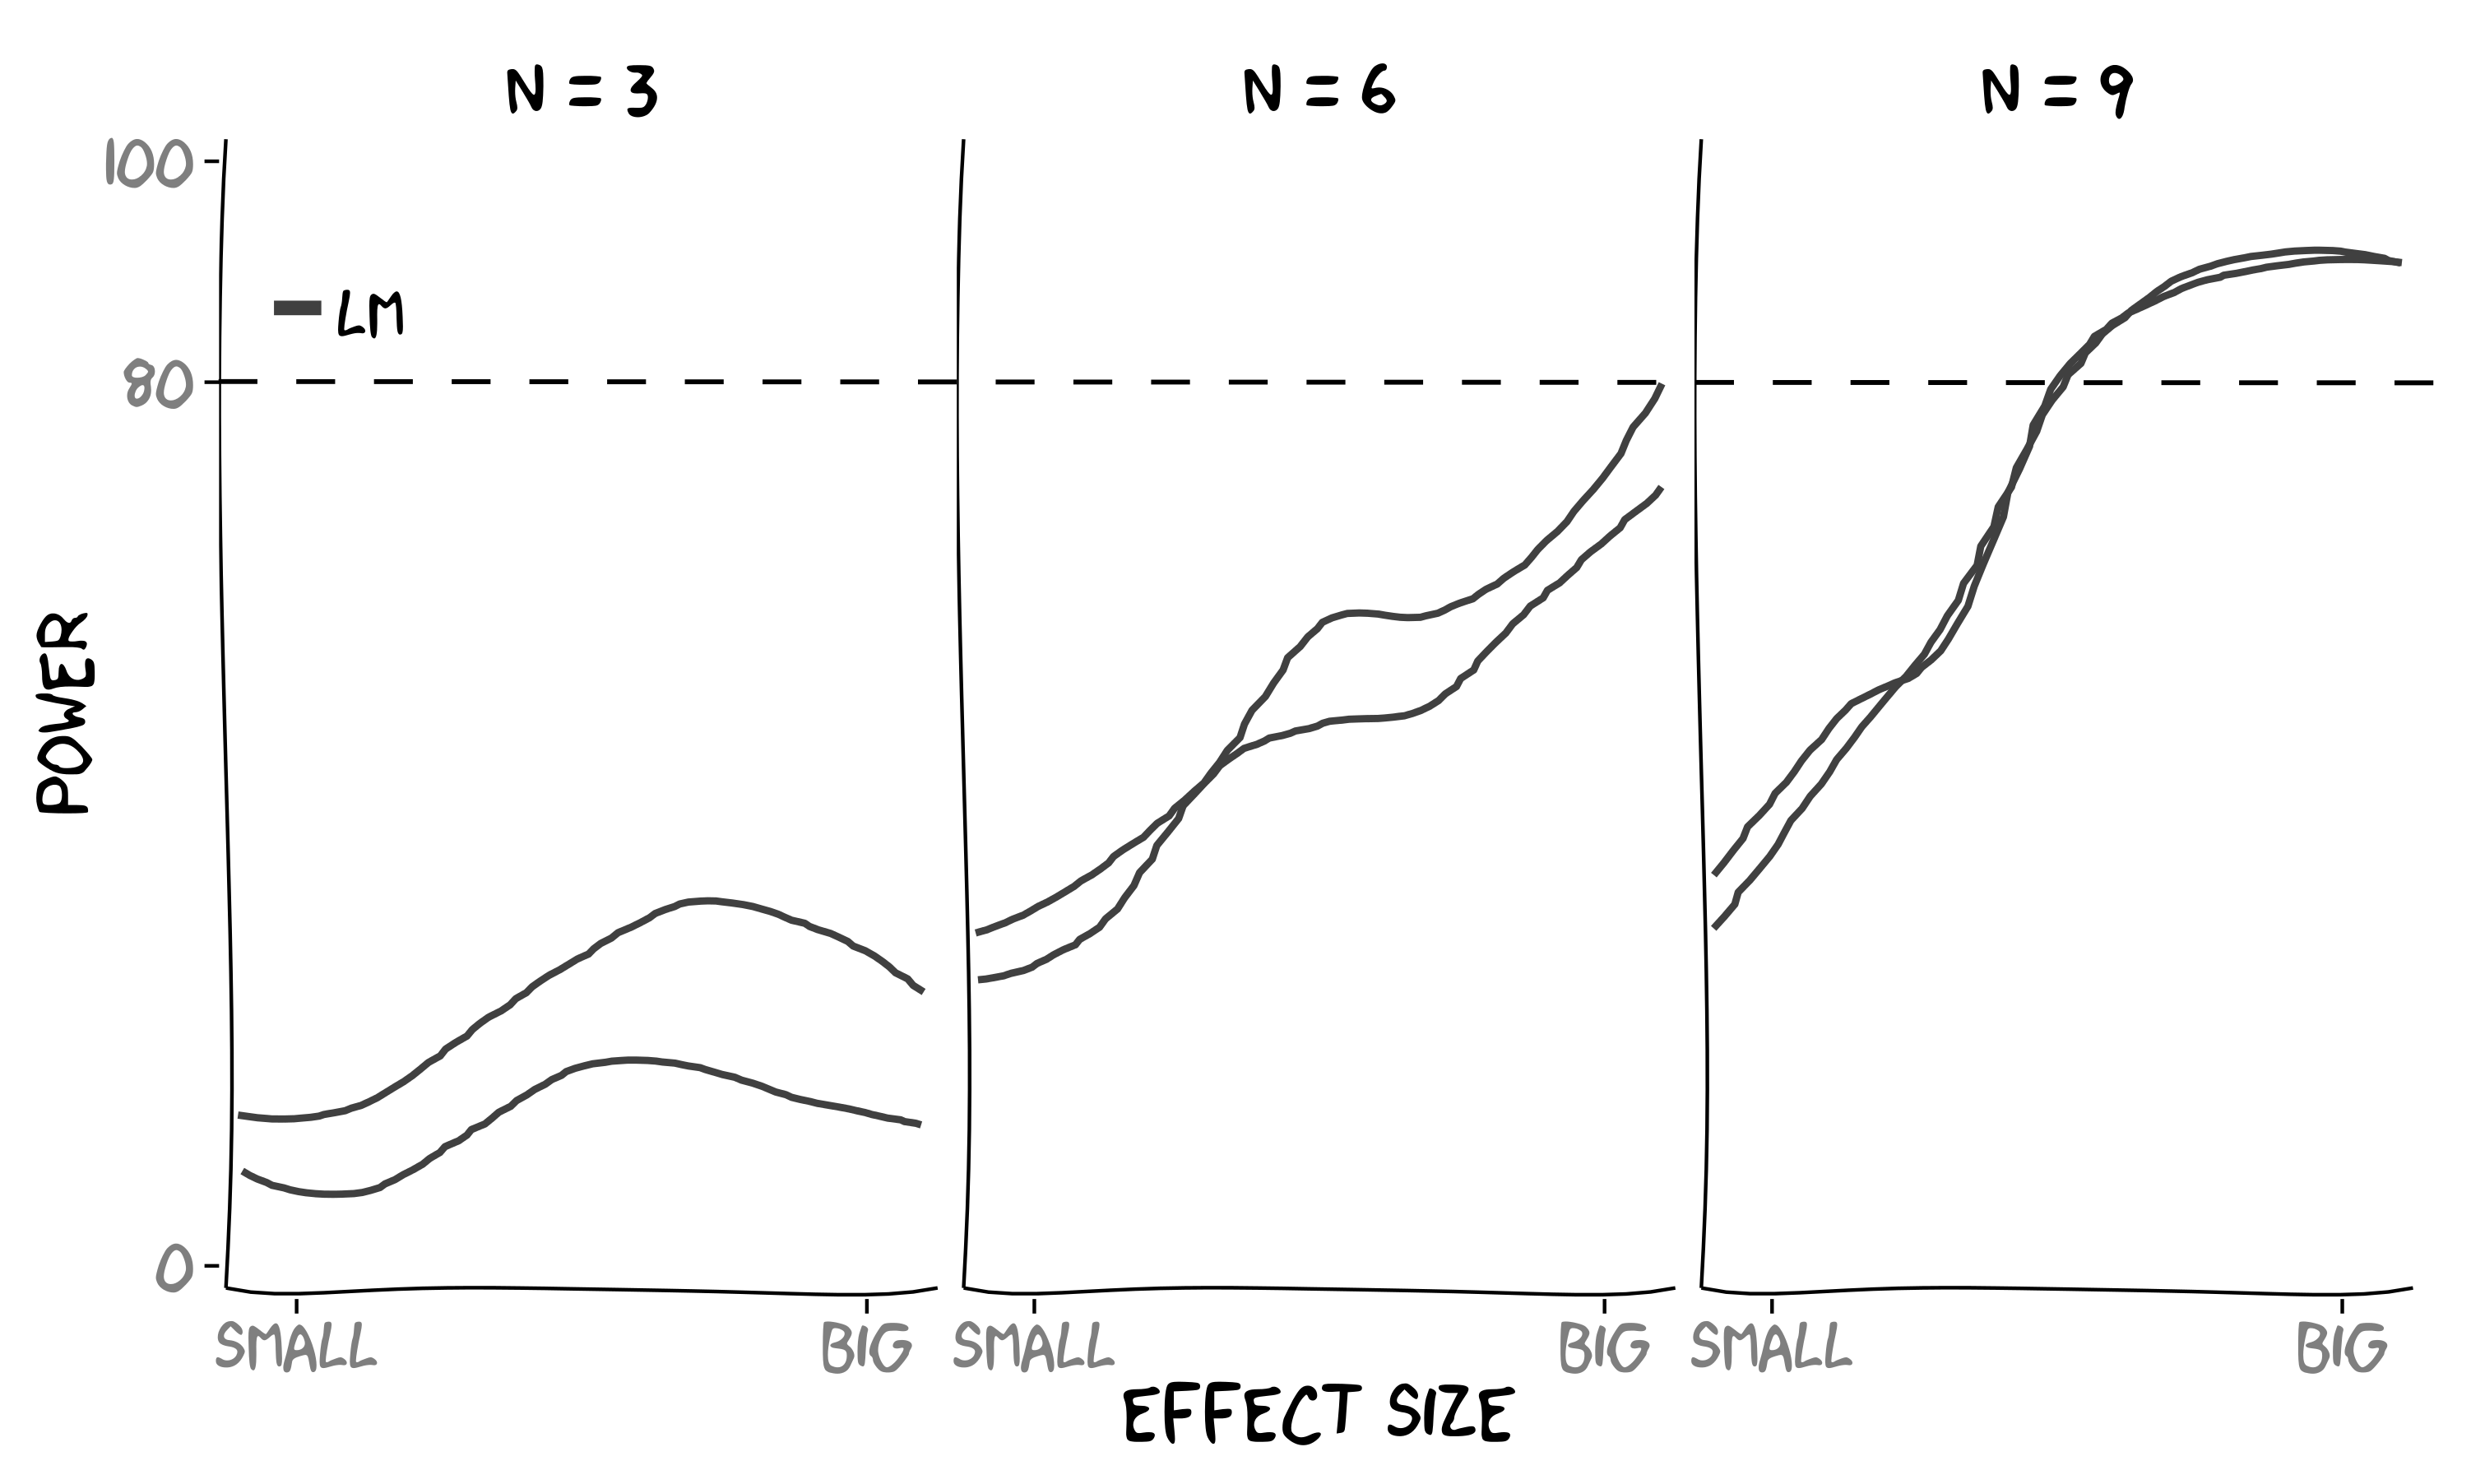
\includegraphics[width = 0.9\textwidth]{fig/glm2.png} \\
\end{frame}


\begin{frame}
\frametitle{Generalized Linear Models can do better}
	\center
	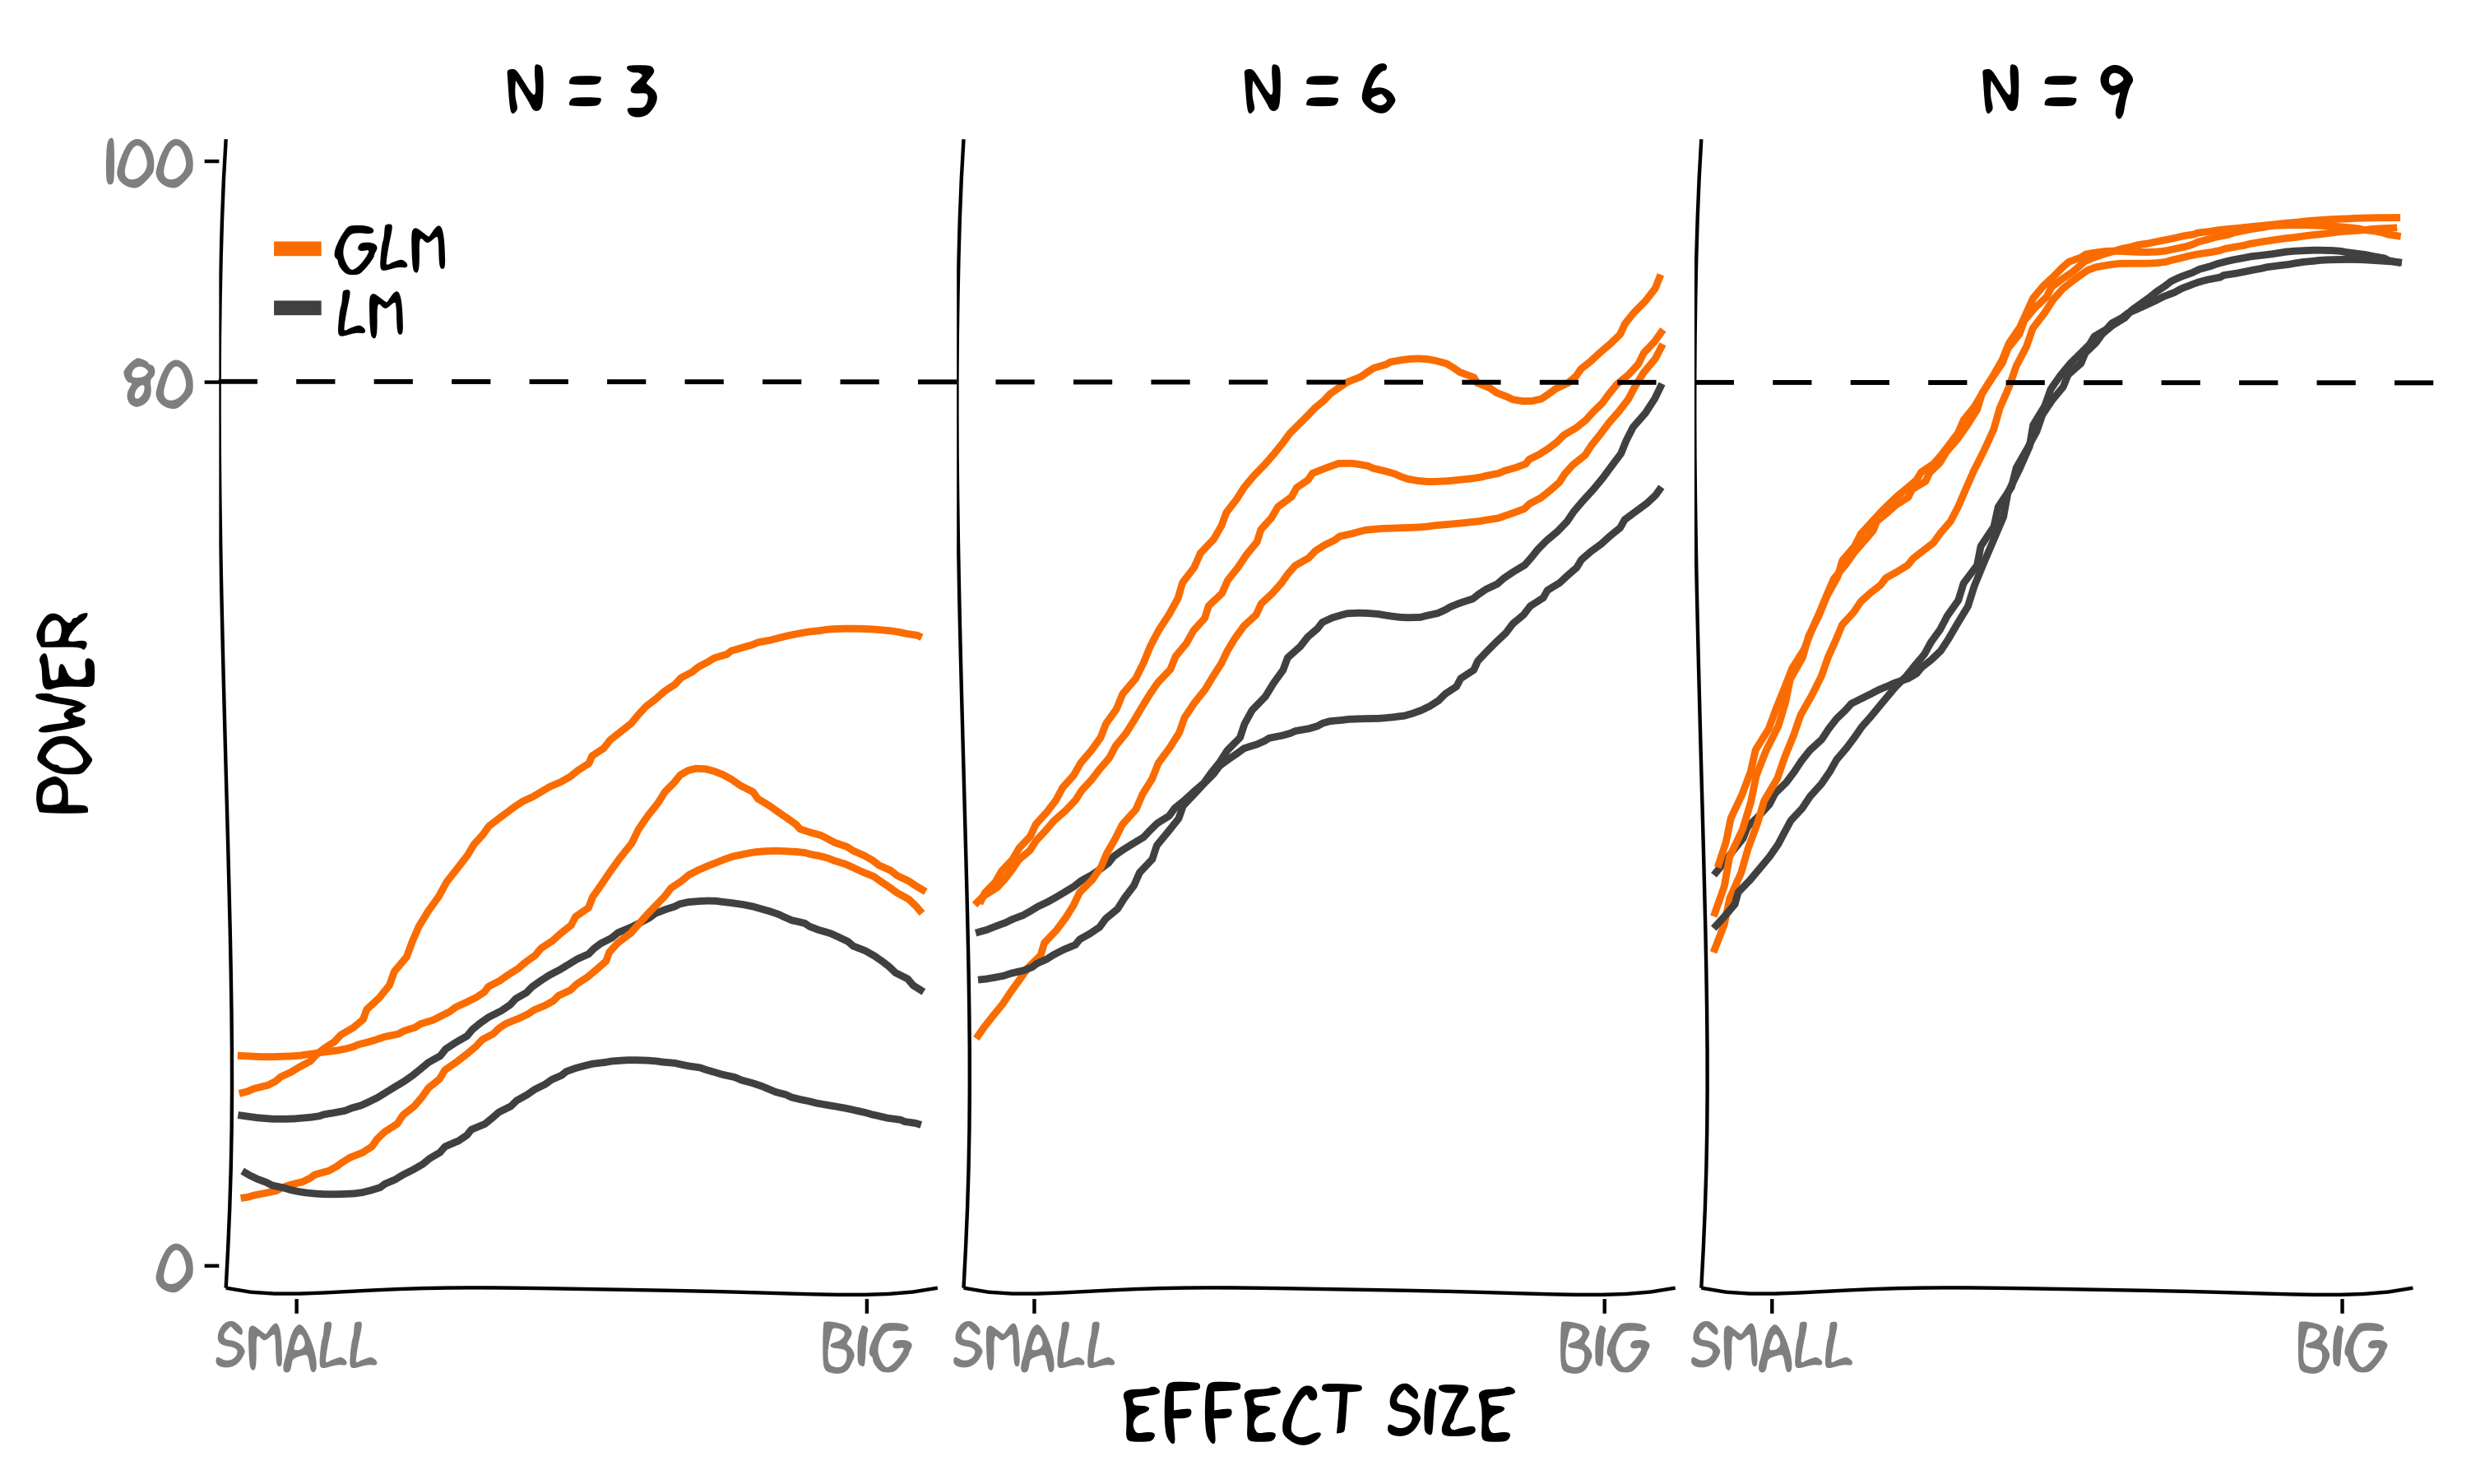
\includegraphics[width = 0.9\textwidth]{fig/glm1.png} \\
	\pause
	\center
	Better abandon NOEC and use a regression design \textsuperscript{1}...\\
	\tiny \textsuperscript{1} debated since 30 years.
\end{frame}



%%% ---------------------------------------------------------------------------
\section{Monitoring Data}
\subsection{}

\begin{frame}[plain]
	\begin{tikzpicture}[overlay, remember picture]
	\node[anchor=center] at (current page.center) {
		\begin{beamercolorbox}[center]{title}
	     \Huge Monitoring Data
	  \end{beamercolorbox}};
	\end{tikzpicture}
\end{frame}


\subsection{}
\begin{frame}
\frametitle{Monitoring data...}
	\begin{itemize}
	\item ... provides an opportunity to study large-scale dynamics of pesticides
	\pause
	\item ... provides the biggest amount of data available
	\pause
	\item ... is really messy
	\end{itemize}
	\begin{center}
	\colorbox{white}{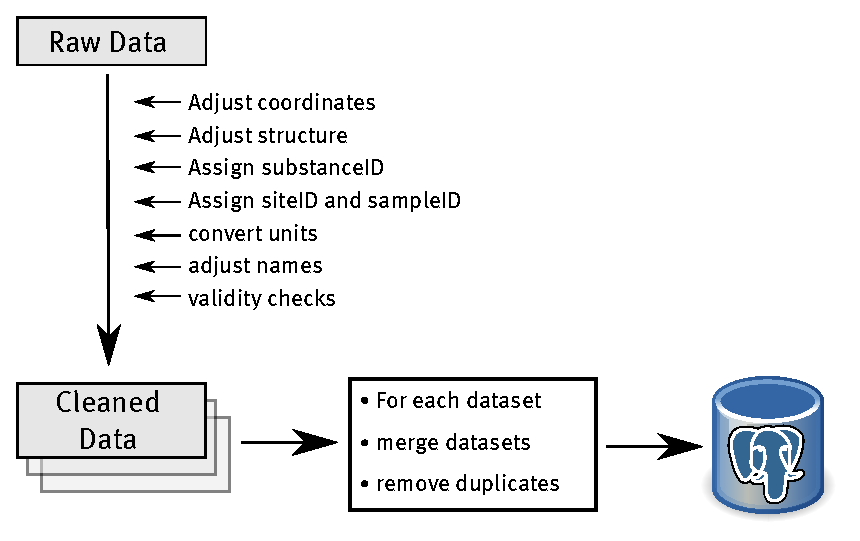
\includegraphics[width = 0.6\textwidth]{fig/data_cleaning.pdf}}
	\end{center}
\end{frame}


\begin{frame}
\frametitle{The biggest currently available dataset on}
	\begin{columns}[t]
	\column{.48\textwidth}
	pesticides
	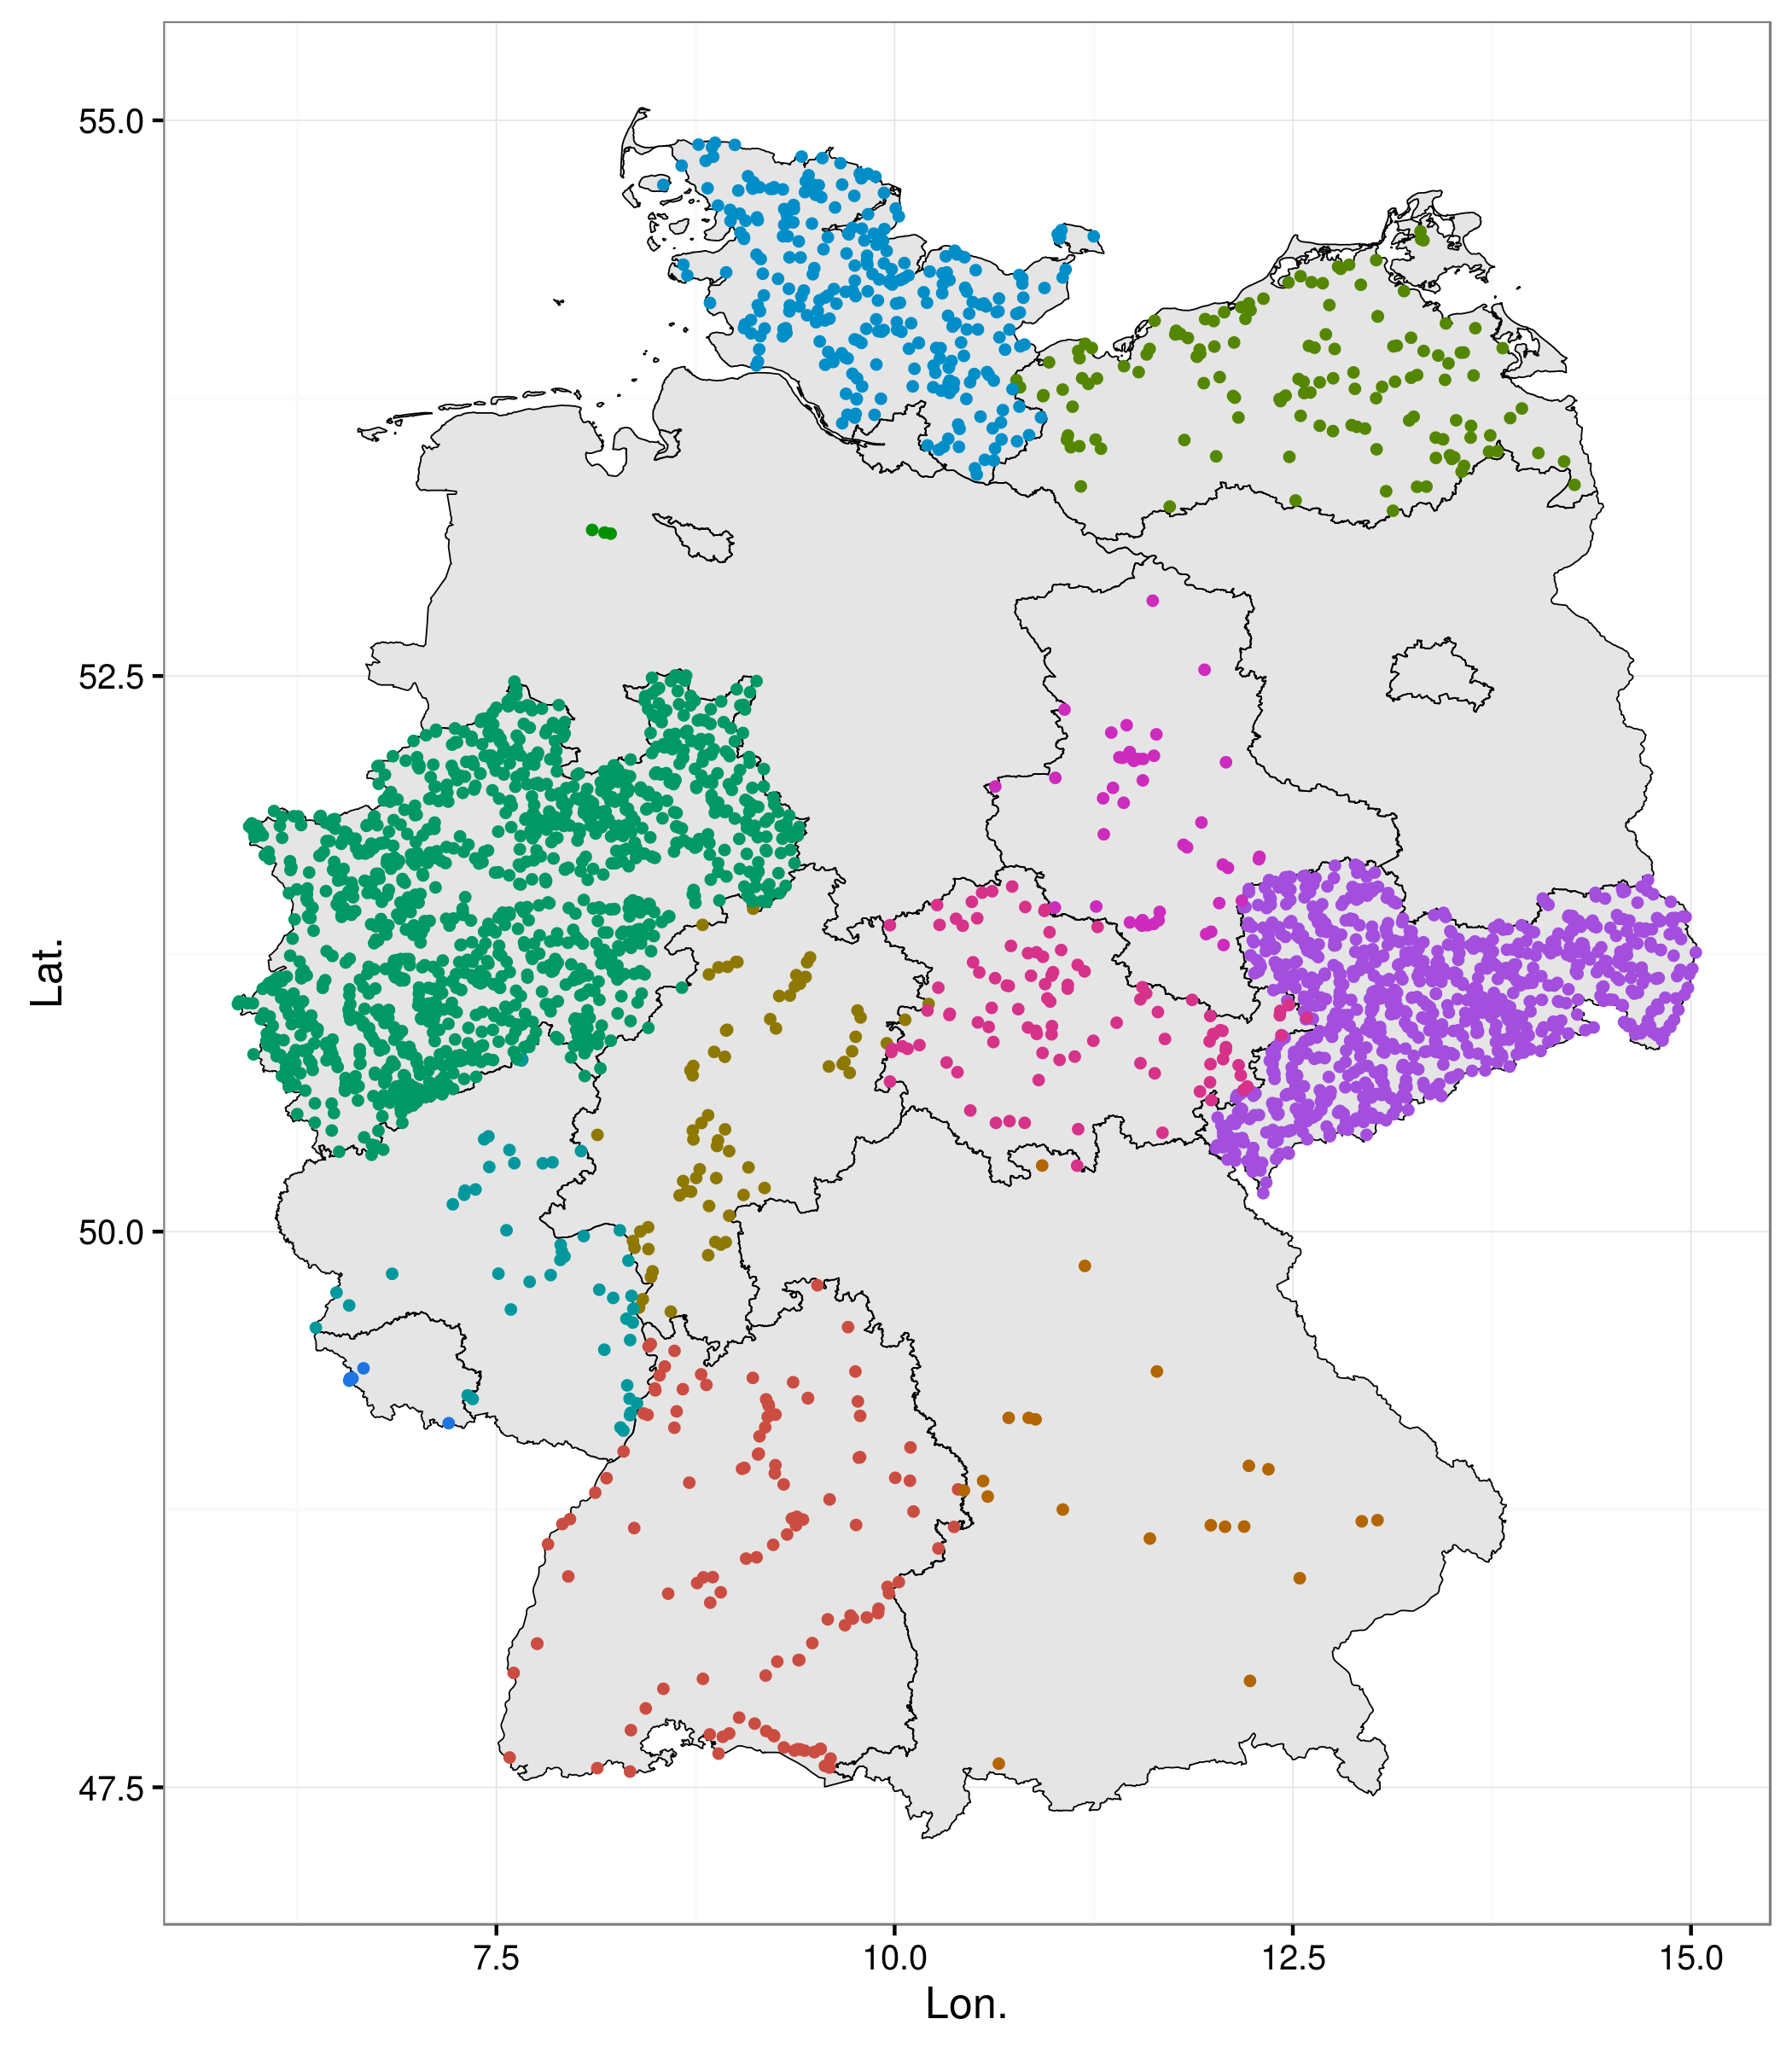
\includegraphics[width = \textwidth]{fig/phch_map.png} \\
	3,000 sites, 45,000 samples, 500 pesticides
	\column{.48\textwidth}
	invertebrates
	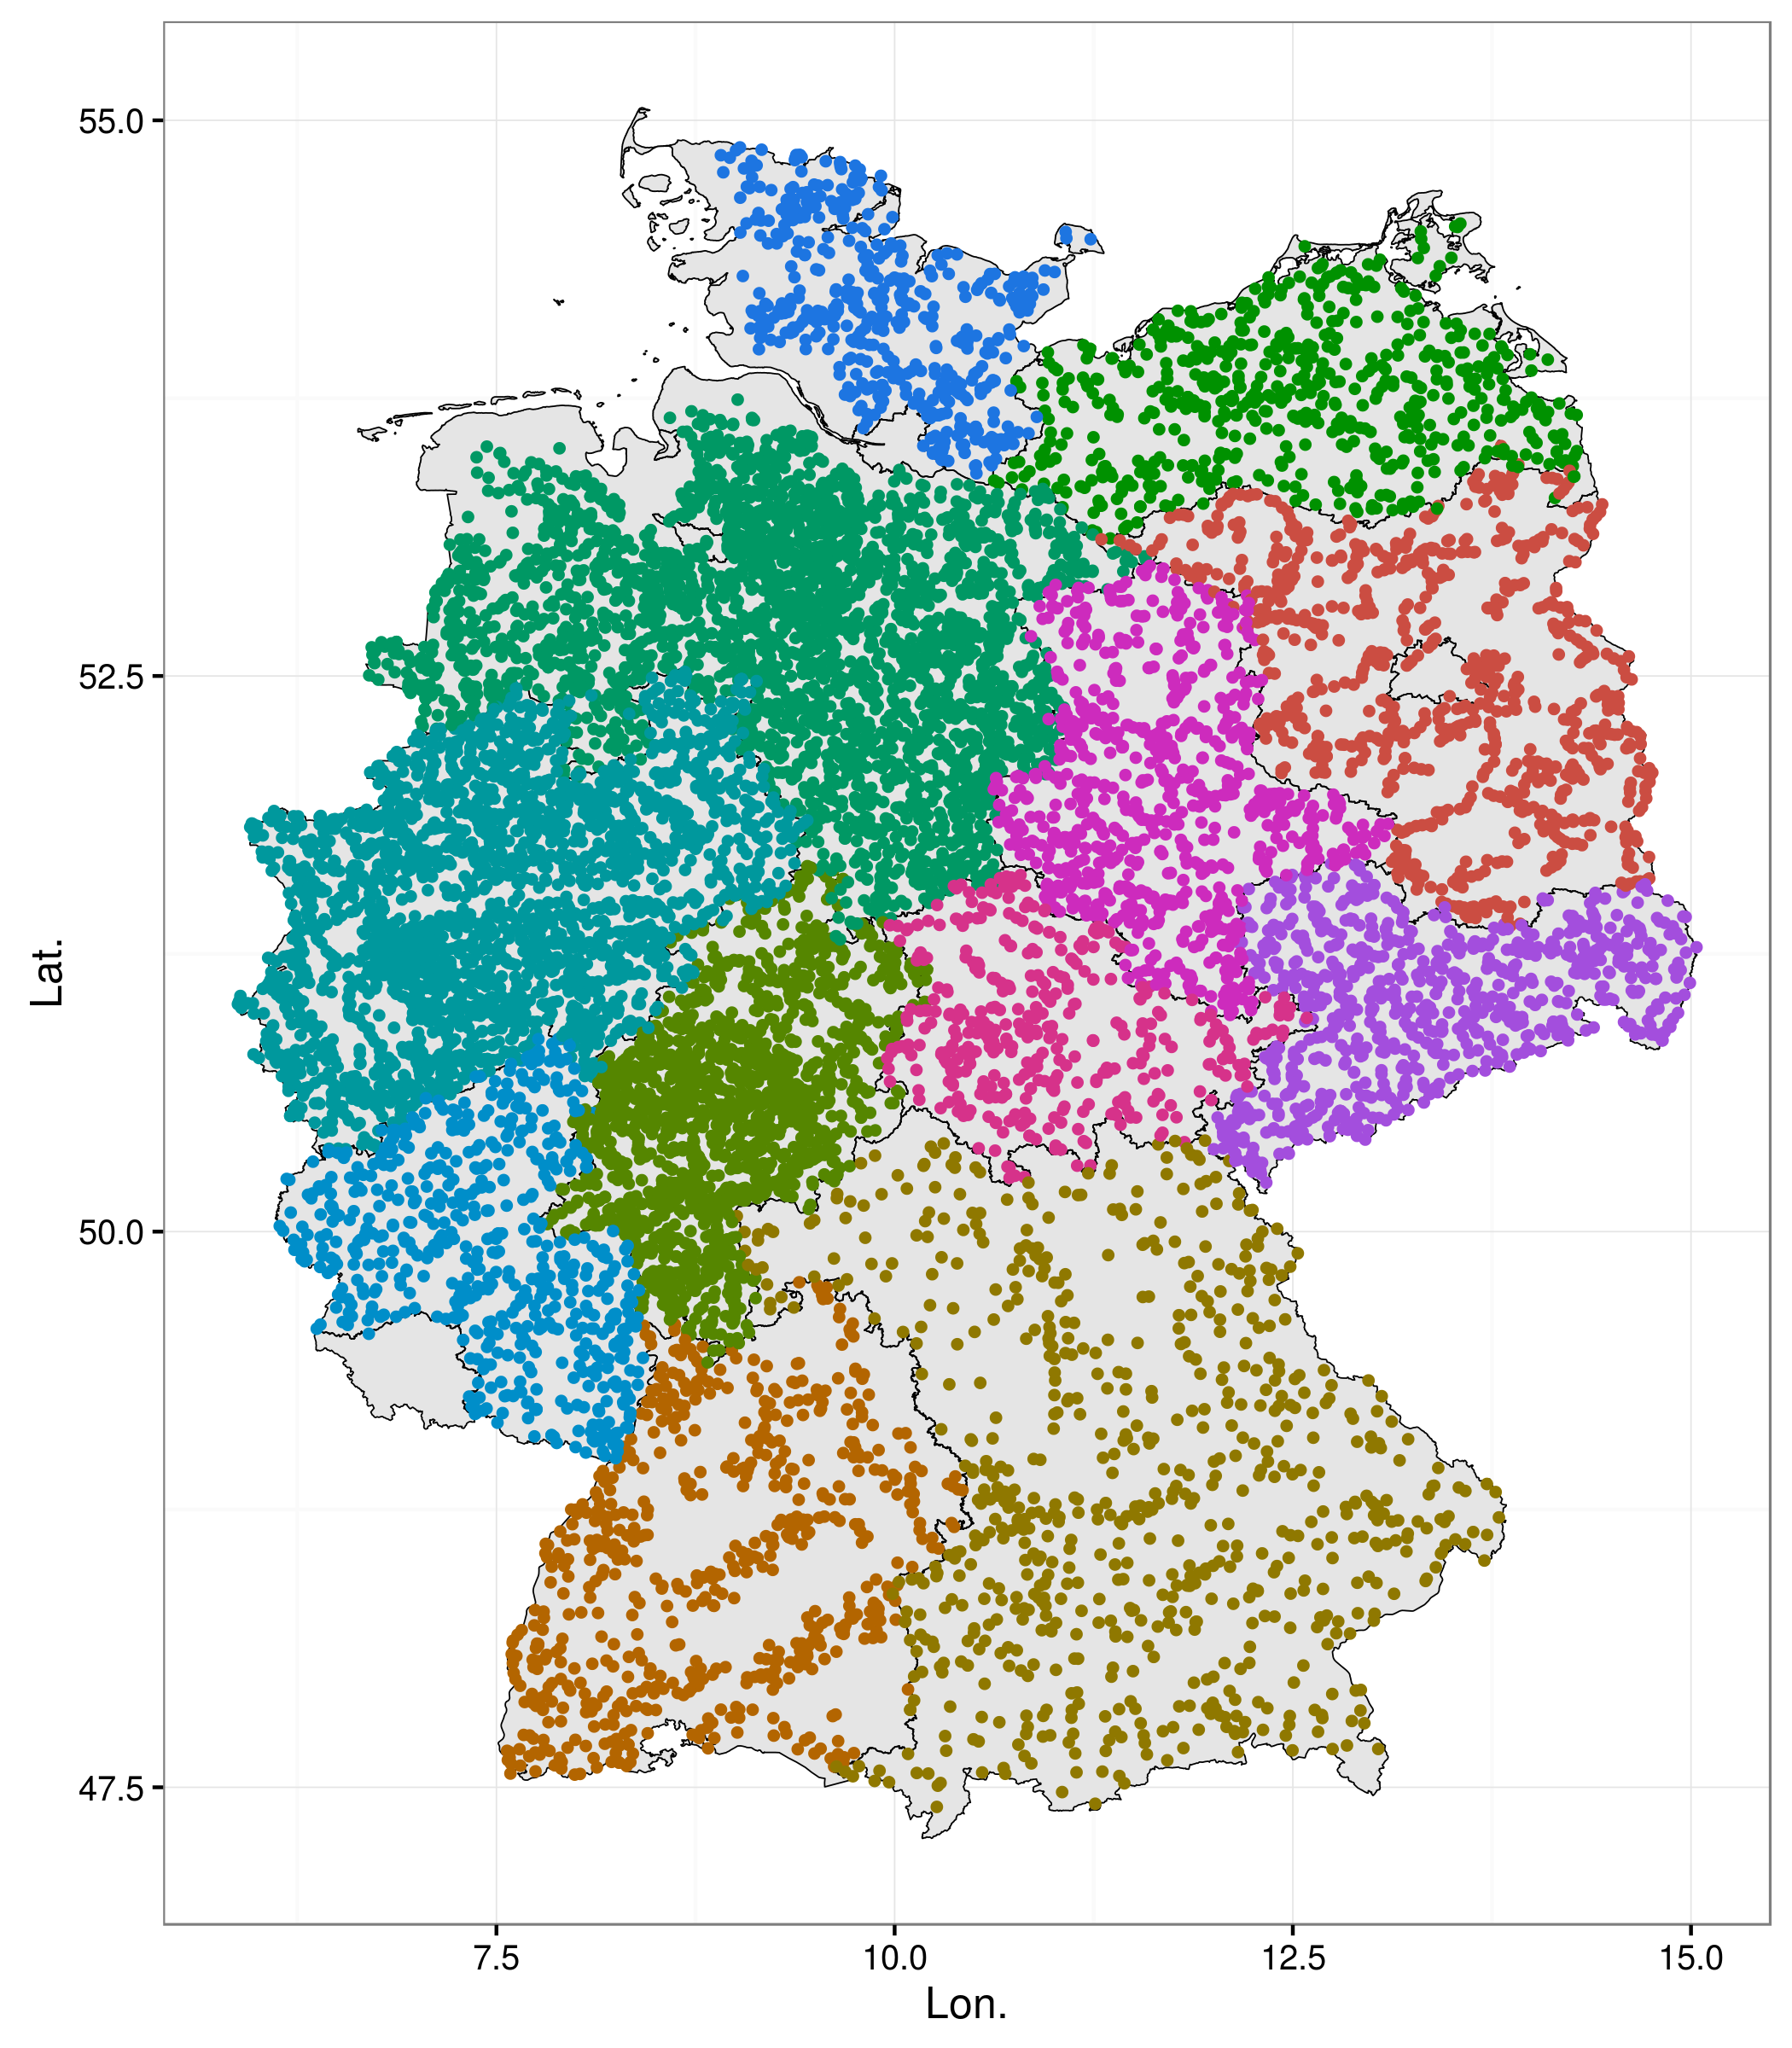
\includegraphics[width = \textwidth]{fig/mzb_map.png} \\
	14,000 sites, 27,000 samples, 3000 taxa
	\end{columns}
\end{frame}


\begin{frame}
\frametitle{Additional data on}
	\textcolor{hilight}{Sites}
	\begin{itemize}
	\item catchment size
	\item agriculture within catchment
	\end{itemize}

	\pause
	\textcolor{hilight}{Samples}
	\begin{itemize}
	\item daily precipitation
	\end{itemize}

	\pause
	\textcolor{hilight}{Compounds}
	\begin{itemize}
	\item RAC, LC50, EQS
	\item chemical group
	\item identifiers
	\item properties
	\end{itemize}
\end{frame}



\begin{frame}
\frametitle{Results - Thresholds}
	\pause
	\begin{center}
		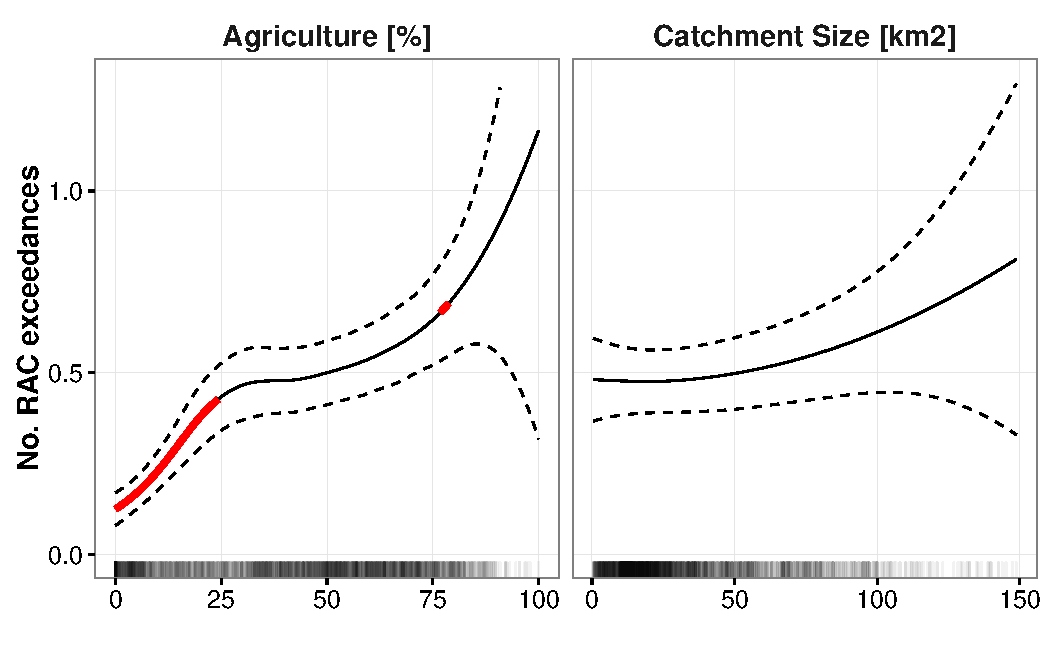
\includegraphics[width = 0.8\textwidth]{fig/figure4.pdf}
	\end{center}
\end{frame}


\begin{frame}
\frametitle{Results - Precipitation \& Seasonality}
	\begin{columns}[T]
	\column{.48\textwidth}
	\begin{itemize}
		\item<1-> Used a mixture model \scriptsize
		$
		RQ_i \sim ZAGA(\mu_i, \sigma, \pi_i) = 
		  \begin{cases}
		    (1 - \pi_i)   & \quad  \text{if } y < LOQ \\
		    \pi_i \times f_{Gamma} (\mu_i, \sigma) & \quad \text{if } y \ge LOQ \\
		\end{cases}
		$
		\normalsize
		\item<2-> Precipitation and Quarter as predictors
		\item<2-> Site within state as random intercept
		\item<3-> \textcolor{hilight}{Precipitation before sampling increases RQ}
		\item<4-> \textcolor{hilight}{Summer higher RQ, but compound specific}
	\end{itemize}
	\column{.48\textwidth}
	\includegraphics<3->[width =\textwidth]{fig/figure5.pdf}
	\end{columns}
\end{frame}


\begin{frame}
\frametitle{Results - Small Water Bodies (SWB)}
	\begin{columns}[T]
	\column{.48\textwidth}
		\begin{itemize}
		\item<1-> most streams are \emph{small}
		\item<1-> refuge of biodiversity
		\item<1-> High risk of pollution
			\begin{itemize}
				\item adjacency to fields
				\item low dilution
			\end{itemize}
		\item<2-> \textcolor{hilight}{Neonicotinoids}
		\item<2-> \textcolor{hilight}{up to 244x RAC}
		\item<2-> \textcolor{hilight}{ecological effects likely}
		\end{itemize}
	\column{.48\textwidth}
	\includegraphics<2->[width = \textwidth]{fig/figure6.pdf}
	\end{columns}
\end{frame}



%%% ---------------------------------------------------------------------------
\section{Software}
\subsection{}

\begin{frame}[plain]
	\begin{tikzpicture}[overlay, remember picture]
	\node[anchor=center] at (current page.center) {
		\begin{beamercolorbox}[center]{title}
	     \Huge Software
	  \end{beamercolorbox}};
	\end{tikzpicture}
\end{frame}

\subsection{}
\begin{frame}
	\frametitle{Biologists and Chemists face similar problems...}
	\footnotesize

	\centering
	\textbf{\textcolor{hilight}{Names}}
	\begin{columns}[t]
	\column{.45\textwidth}
	\emph{Osmia rufa, Osmia bicornis, Osmia ruffa, Osmia unilandauis, Osmia spec.} 
	\column{.45\textwidth}
	Chlorpyrifos, Chlorpyriphos, Chlorphyrifos, Chlorpyrifos-ethyl, Chlorpypifot
	\end{columns}
	\pause

	\centering
	\textbf{\textcolor{hilight}{Hierarchies}}
	\begin{columns}[t]
	\column{.45\textwidth}
	Hymenoptera/ Apoidea/ Megachilidae/ Osmia/ rufa 
	\column{.45\textwidth}
	organophospate, ester, insecticide
	\end{columns}
	\pause

	\centering
	\textbf{\textcolor{hilight}{Attributes}}
	\begin{columns}[t]
	\column{.45\textwidth}
	Wing length, Mass, Season 
	\column{.45\textwidth}
	Mass, $K_{OW}$, $LC_{50}$
	\end{columns}
	\pause

	\centering
	\textbf{\textcolor{hilight}{Identifiers}}
	\begin{columns}[t]
	\column{.45\textwidth}
	NCBI, ITIS, EOL, ... 
	\column{.45\textwidth}
	2921-88-2, Clc1c(OP(=S)[...], InChI=1S/C9H11C[...], SBPBAQFW[...], CSID,...
	\end{columns}
	\vspace{0.8em}
	\pause

	\rule{\textwidth}{1pt}
	\textbf{\textcolor{hilight}{Amount of data}}

	\begin{columns}[t]
	\column{.45\textwidth}
	\centering
	2993 taxa
	\column{.45\textwidth}
	\centering
	489 pesticides \\ (+ 590 other organics)
	\end{columns}
\end{frame}


\begin{frame}
	\frametitle{Instead of wasting time...}
\onslide<2->{
	\textbf{\textcolor{hilight}{taxize - taxonomic search and retrieval in R}}
	
\includegraphics[width=0.6\textwidth]{fig/taxize_twitter.png}
}
	\vfill
\onslide<3->{

	\hfill
\includegraphics[width =.6\textwidth]{fig/sources.png}
	}
\end{frame}



\begin{frame}
	\frametitle{Instead of wasting time...}
\onslide<2->{
	\emph{''\textcolor{hilight}{webchem} ...likely saved hundreds of working hours''}
	}
\onslide<3->{
	\begin{center}
	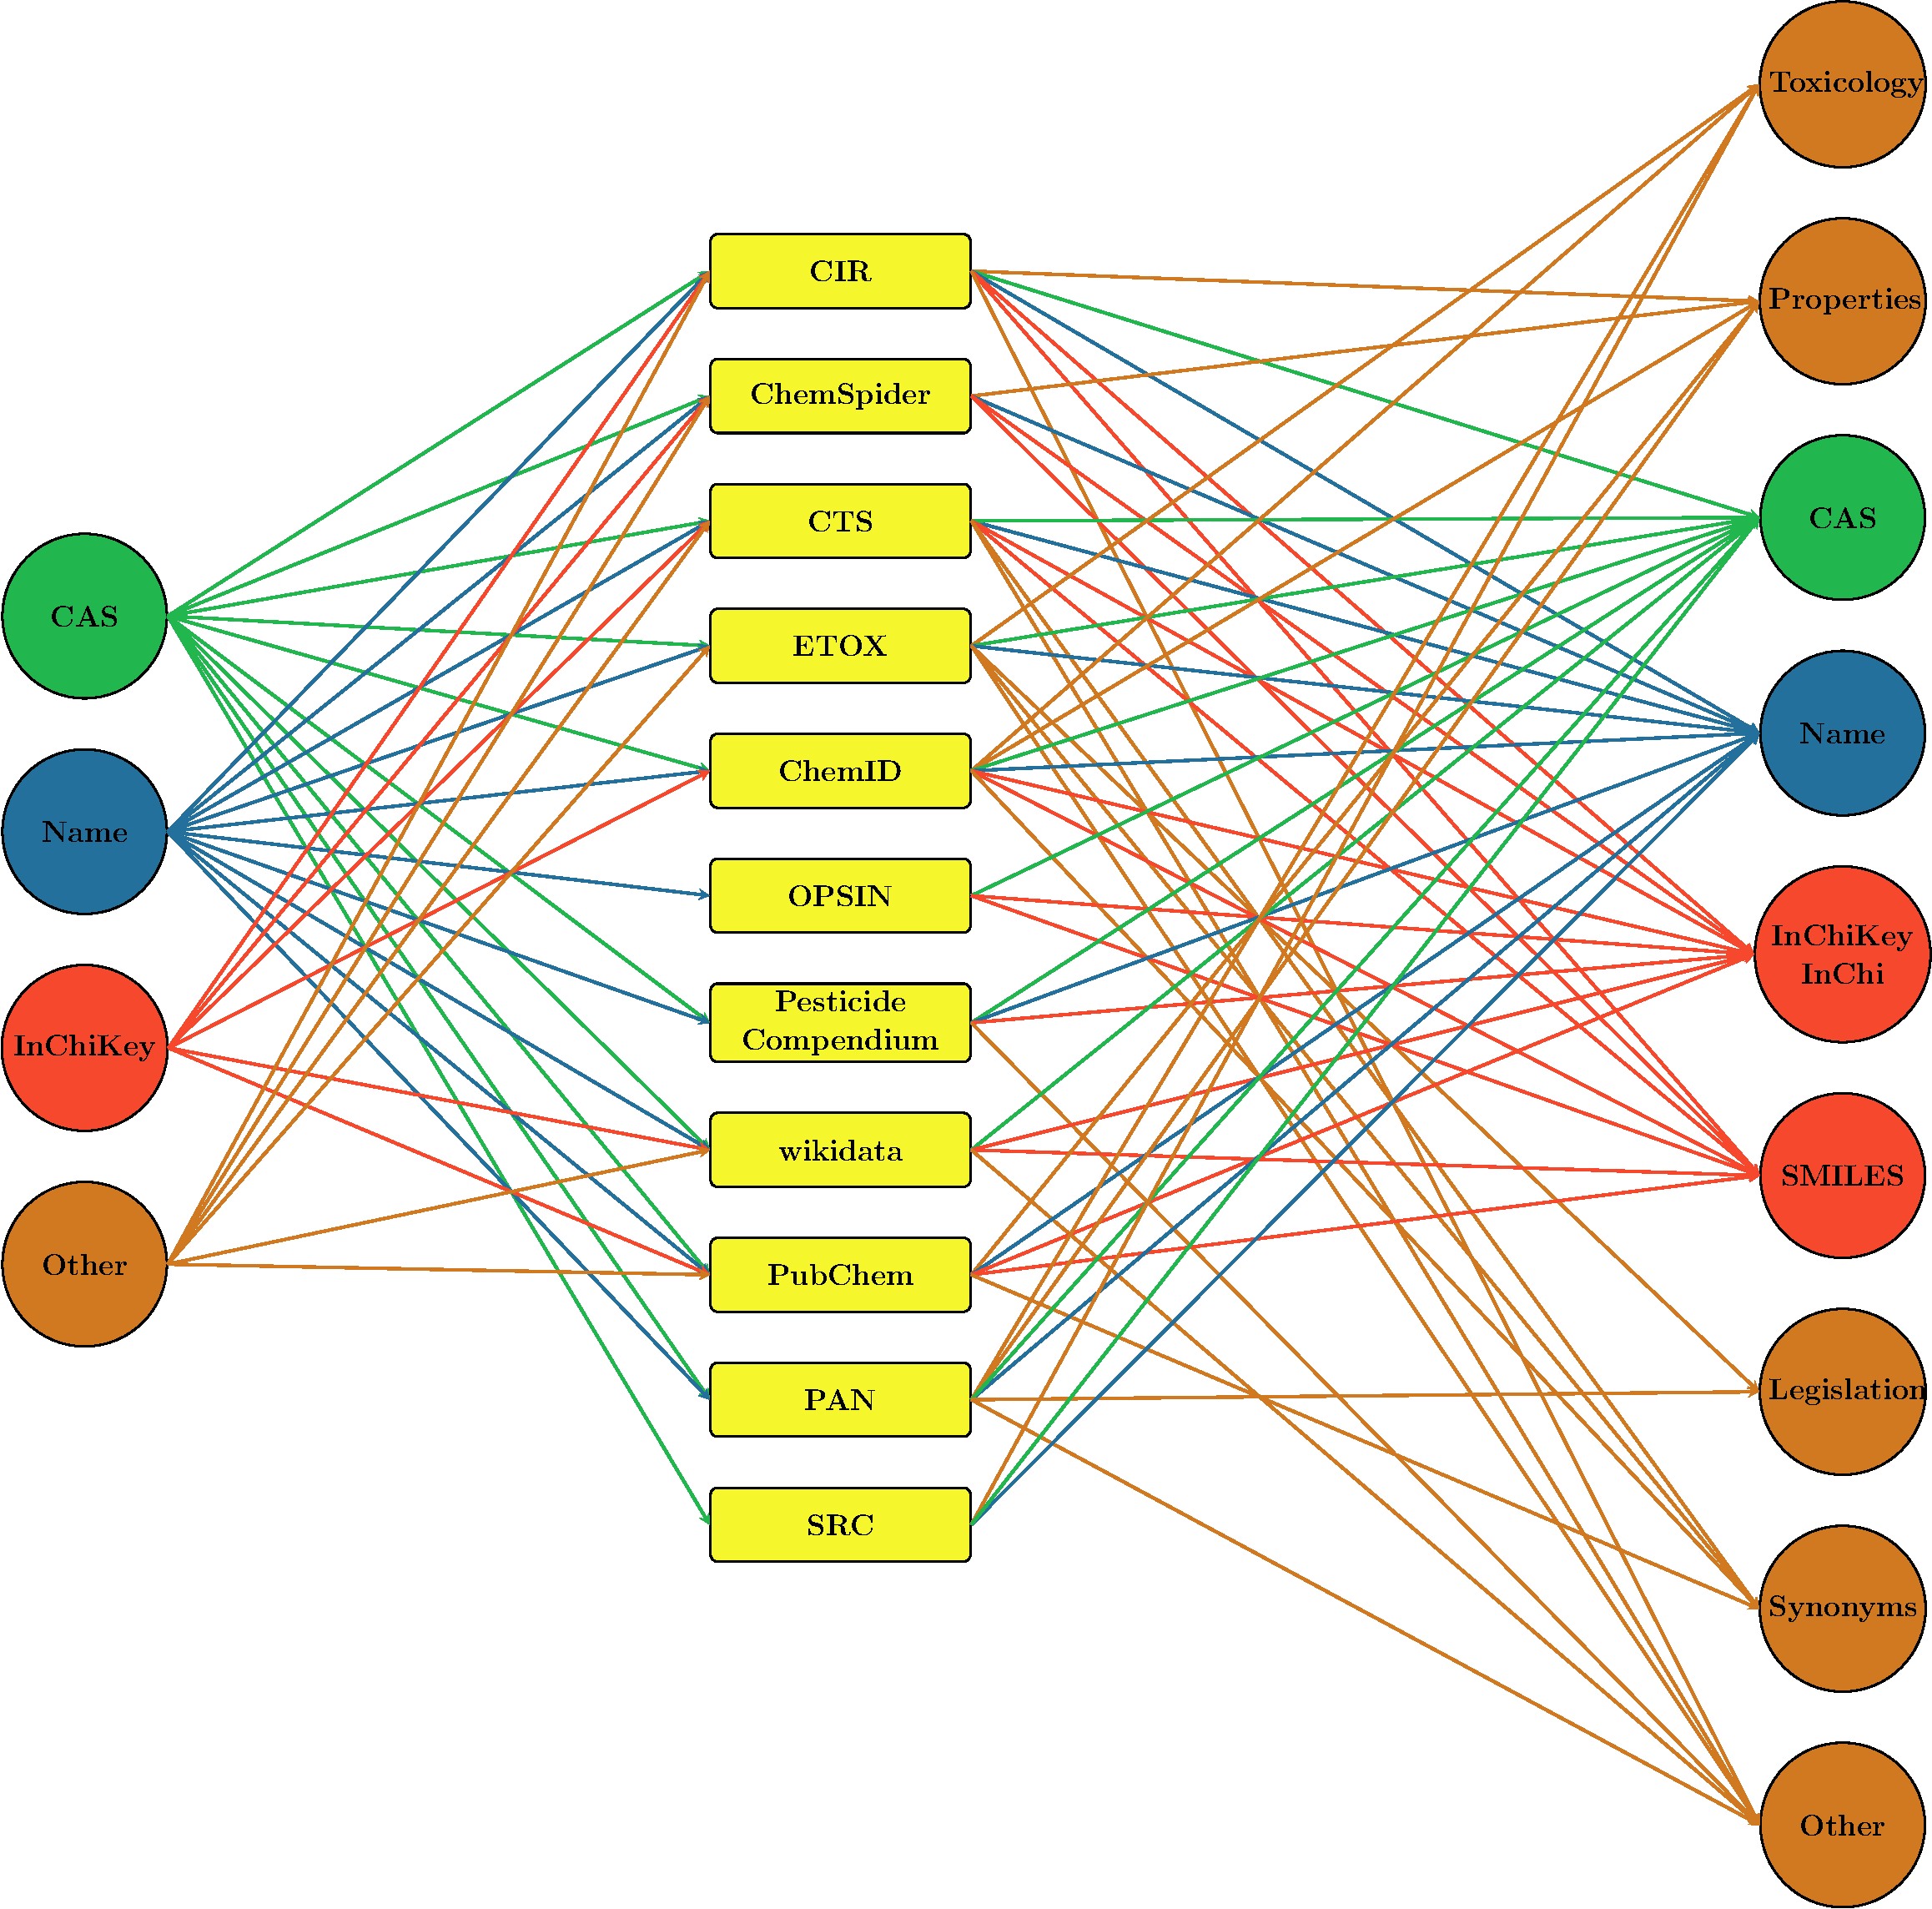
\includegraphics[width =.7\textwidth]{fig/fig1.pdf} \\
	\end{center}
	}
	\vspace*{-1.5cm}
	\hfill 
\onslide<2->{
	\tiny Münch (2016)
	}
\end{frame}





%%% ---------------------------------------------------------------------------
\section{Outlook}
\subsection{}

\begin{frame}
	\frametitle{Conclusions from my PhD}
	\begin{itemize}
	\item Change your model, not your data
	\pause
	\item Ultimately ban NOEC
	\pause
	\item Monitoring data can be used to 
			\begin{itemize}
				\item study pesticide dynamics
				\item inform ERA
			\end{itemize}
	\pause
	\item Agricultural SWB at risk from pesticides
	\pause
	\item Handling big eco(toxico-)logical data not easy 
			\begin{itemize}
				\item now easier
			\end{itemize}
	\end{itemize}
\end{frame}


\begin{frame}[plain]
	\begin{tikzpicture}[overlay, remember picture]
	\node[anchor=center] at (current page.center) {
		\begin{beamercolorbox}[center]{title}
	     \Huge Outlook
	  \end{beamercolorbox}};
	\end{tikzpicture}
\end{frame}


\subsection{}
\begin{frame}
	\frametitle{Analysing chemical concentrations is not easy, because of}
	\begin{columns}[T]
	\column{.4\textwidth}
		\footnotesize
		\vspace{1em}
		\begin{itemize}
		\item continuous distribution in $\mathbb{R}^{+}_0$
		\item censoring \\ (x \textless LOQ )
		\item<2-> non-linearity \\ (season, trends)
		\item<2-> dependency \\(spatial, temporal)
		\item<2-> missing data
		\end{itemize}
	\column{.6\textwidth}
		\colorbox{white}{\includegraphics<1->[width =\textwidth]{fig/glyph.pdf}}
	\end{columns}
\end{frame}



\begin{frame}
	\frametitle{Dealing with censored, non-normal data}
	\includegraphics<1>[width =0.8\textwidth]{fig/p0.pdf}
	\includegraphics<2>[width =0.8\textwidth]{fig/p1.pdf}
	\includegraphics<3>[width =0.8\textwidth]{fig/p2.pdf}
	\includegraphics<4>[width =0.8\textwidth]{fig/p3.pdf}
	\includegraphics<5>[width =0.8\textwidth]{fig/p4.pdf}\\
	\onslide<5-> \textcolor{hilight}{Guidance how to model environmental concentrations is missing}
\end{frame}



\begin{frame}
	\frametitle{Temporal dynamics of pesticide occurrence}
	\begin{itemize}
	\item Pesticides show compound specific dynamics
	\item Mixture dynamics? - Multivariate response. 
	\pause
	\item<2-> Seasonality, Trends (Fade out...)? 
	$y = \beta_0 + f_{seasonal}(x_1) + f_{trend}(x_2) + \epsilon;  \epsilon \sim ???$
	\end{itemize}
	\begin{center}
	\includegraphics<2->[width =0.6\textwidth]{fig/gam1.png}
	\end{center}
\end{frame}




%%% ---------------------------------------------------------------------------
%%% Final slide
\begin{frame}[plain]
	\frametitle{}
	\vspace{1em}
	\begin{centering}
	\Large \textcolor{title}{Statistical Ecotoxicology \\ - Improving the utilization of data for ecological risk assessment} \\[1em]
	Eduard Szöcs \\[0.3em]
	\tiny \textcolor{gray}{Institute for Environmental Sciences, University of Koblenz-Landau} \\[3em]
	\end{centering}
	\normalsize
	\textcolor{hilight}{\faLaptop}~~~\href{http://edild.github.io/}{http://edild.github.io/ }\\[.5em]
	\textcolor{hilight}{\faTwitter}~~~\href{http://twitter.com/EduardSzoecs}{@EduardSzoecs} 	\\[0.5em]
	\textcolor{hilight}{\faEnvelope}~~~\href{mailto:szoecs@uni-landau.de}{szoecs@uni-landau.de} \\[.5em]
	\textcolor{hilight}{\faGift}~~~\href{https://github.com/edild/talk_work2}{https://github.com/edild/talk\_work2}\\[0.5em]
	\hfill 
\includegraphics[width =.3\textwidth]{fig/Cc-by-nc_euro_icon.png} 
\end{frame}
\end{document}
